\documentclass[11pt]{article}
\addtolength{\oddsidemargin}{-1in}
	\addtolength{\evensidemargin}{-1in}
	\addtolength{\textwidth}{2in}
	\addtolength{\topmargin}{-.9in}
	\addtolength{\textheight}{1.5in}

\usepackage{graphicx}
\begin{document}

\begin{enumerate}
\item {\bf Introduction:}
%
\begin{enumerate}
\item 1.1 Purpose of this Document:\newline
This document will be a detailed analysis of the project I will be working during the summer. 
\item 1.2 Scope of this document:\newline
This document covers the core of the system. It includes the code that will do most of the calculations to find suitable schedules, the GUI for the applet, and the requirements for running the applet.
\item 1.3 Overview:\newline
The program is mainly for college students or those just entering college and need to create a schedule for their classes.  The program will allow students to create effective schedules for their classes without becoming a burden.  Also students will be able to fit their courses around their own day to day schedule, instead of fitting their schedule around their courses.
\item 1.4 Business Context:\newline
The Amp program gives students the chance to experience researching and using resources that are available to them, especially for minorities.  It helps students prepare for graduate school.\newline
\end{enumerate}

\item {\bf General Description:}
\begin{enumerate} 
\item 2.1 Product Functions:\newline
		The system should be able to take in multiple classes with different time slots, create a unique schedule out of every possible combination of classes, then display the schedules that have no conflicting time slots.  The system should also be able to take in other schedules, such as work or any times the student would not like to have class, and determine whether it will conflict with the course schedule.
The system should make it effortless for GMU students to create class schedules that will not interfere with their daily lives.  The system should not jeopardize ease of use for performance.
\item 2.2 Similar System information:\newline
		The product will be used along side a website that will hold the system.  The system will be a web applet. If we can finish the project before the deadline we might be able to turn it into a web application.
\item 2.3 User Characteristics:\newline
		Users do not need prior experience to run the software, but should be familiar with how scheduling works and day to day applications.
\item 2.4 User Problem Statement:\newline
		In order to use the software, users will need to have prepared the classes they would like to schedule which might be difficult.  Users will have to input every single potential timeslot which might become time consuming.
\item 2.5 User Objectives:\newline
		Users will want an easy and fast way to input their courses and the individual timeslots.  Inputting so many different timeslots can become very tedious, so the GUI would need to lessen this task.
We can do this by asking for the class name once, then create textboxes for the users to input different times.  A combo box might be best for the minutes.
Finally the schedule should be displayed in a manner that is easy to read and comprehend.  Somewhat like a calendar.
\item 2.6 General Constraints:\newline
		Since the program will be a web applet it will not have access to system resources, so we cannot save files or run programs on the user�s computer.  We will also need to make the program reusable incase we want to turn it into a stand alone application or a web application.\newline
\end{enumerate}

\item {\bf Functional Requirements:}
\begin{enumerate}
\item System must be able to compute working schedules efficiently and in a timely manner.
		\begin{enumerate} 
		\item Description:\newline
			The applet should not take long to load the working schedules and display them to the user.
		\item Criticality:\newline
			Very critical
		\item Technical issues:\newline
			System will have to not only compare each course but also its labs.  It will also have to compare the final schedules with other the timeslots the student would not like to have class.
		\item Risks:\newline
			If the user inputs wrong data, such as replacing the start time of a course with its end time, the system will not be able to process it.
		\end{enumerate}
		
\item System should be able to store the data temporarily.
		\begin{enumerate} 
		\item Description:\newline
			If the user wants to go back and enter another class or change a timeslot, he should not have to enter all the data in again.  The user should be able to go back to his previous courses easily.
		\item Criticality:\newline
			Very critical.
		\item Technical issues:\newline
			The system will have to somehow display the current courses and timeslots in a way that is easy for the user to read and change.
		\item Risks:\newline
			none\newline
		\end{enumerate}

\item GUI should display the final results in a manner that is readable.
		\begin{enumerate}
		\item Description:\newline
			After the program calculates the working schedules, it should display a chart containing a schedule.  As the user looks through the schedules the chart should redisplay the current schedule that the user is looking at.\newline
			The chart that is displayed should highlight the classes and the times that the user listed as not wanted.
		\item Criticality:\newline
			Very Critical.
		\item Technical issues:\newline
			I am very bad with GUI designs.
		\item Risks:\newline
			Fitting the chart with a schedule that has a lot of classes, in a predetermined size box.
		\end{enumerate}

\item The program should ask for classes that are optional for the student.
		\begin{enumerate}
		\item Description:\newline
			Some classes students are not sure whether they should take them or not depending on their schedule.  The system should show any schedule that contains or does not contain the optional classes.
		\item Criticality:\newline
			Somewhat critical.
		\item Technical issues:\newline
			Applet should have a check box, that users can check if the class is optional.
		\item Risks:\newline
			If there are too many optional classes it will greatly increase the time it takes to calculate the resulting schedules.\newline
		\end{enumerate}
\end{enumerate}
			
\item {\bf Interface Requirements:}
	\begin{enumerate}
	\item 4.1 User Interfaces:\newline
		The system will interface with the user mainly through the GUI.
	\item 4.1.1 GUI:
		\begin{itemize}
		\item The graphical user interface will first present the user with a couple of text boxes and combo boxes for the user to input the class name and its timeslots.  It will also have 4 buttons, NEXT, PREVIOUS, REMOVE, and ADD, which will add that class to the list.
			\begin{itemize}
			\item This will also contain check boxes next to the classes.  The user can check these if the class is optional. 
			\item It will also have a PANEL that displays the classes that were added.  The user can click on any of these to highlight a class, and change its properties.
			\end{itemize}
		\item The next phase, the GUI will present the user with similar boxes for the user to input when he would not be available for classes. 
			This phase might have a chart that the user can use to enter when he is unavailable instead of textboxes.
		\item The third phase, will display the resulting schedule to the student.  It will have a PREVIOUS button incase the student wants to change any class.
		\end{itemize}
	\item 4.1.2 API:\newline
		To be filled later.\newline
	\end{enumerate}

\item {\bf Performance Requirements:}\newline
	Since the system will be an applet the user will only need an internet connection.  If we make it a stand alone application, then the user will need a java virtual machine.\newline

\item {\bf Design Constraints:}
	\begin{itemize}
	\item If the system will save user�s schedules for later use, the information cannot be shown to any other users.
	\item If user is to be asked for any personal information, the system will need a way to obtain proof of the user's permission.
	\item System does not have access to the user's computer so it will need some other way of storing the user's information and previous schedules.  We can do this by using a database or asking the user if he would like to save or download his current work.
	\end{itemize}

\item {\bf Other Non-Functional Attributes:}
	\begin{enumerate}
	\item Security will not be a major issue, unless we will be keeping a database of all the users and their saved work.  That will not be covered by this SRS.
	\item Reliability will be a great issue in the system, mainly because many students will be using it to schedule their classes and small mistakes can greatly effect a student's standing.\newline
	System must be able to keep track of the user's progress, incase an error occurs.
	\item System should also be extensible since it will probably go through a lot of changes.  Features and updates should be easy to setup, without having to change to much in the code.
	\end{enumerate}
	
\item {\bf Premiliminary Object-Oriented Domain Analysis:}
	\begin{enumerate}		
	\item Class Descriptions: (Course)
		\begin{enumerate}
			\item {\it CLASS NAME:} Course
			\item Concrete
			\item {\it PURPOSE:} This class will hold a single course. It will also include the course's name, section, and three different timeslots.
			\item {\it COLLABORATIONS:}
				\begin{itemize}
					\item This class holds three TimeSlots.  The time slot will hold the actual time and days for each course.  Each course can have a lab, lecture, and recitation, so each one will have a seperate TimeSlot.
				\end{itemize}
			\item {\it ATTRIBUTES:}
				\begin{itemize}
					\item String name
					\item int section
					\item TimeSlot lab;
					\item TimeSlot lecture;
	    		\item TimeSlot recitation;		
				\end{itemize}
			\item {\it OPERATIONS:}
				\begin {itemize}
					\item getTimeSlot(integer type); returns: TimeSlot \newline
					User can ask for the object reference to one of the TimeSlots.  The argument specifies which TimeSlot he wants.
					\item getLabTime(integer point); returns: integer \newline
					User can ask what time a TimeSlot begins or ends. Point specifies if the he wants the start time or the end time of the TimeSlot and point must be either 0 or 1. "`getRecitationTime and getLectureTime are the same methods.
					\item setLabTime(String time, String days) \newline
					Allows the user to set the time slot for a lab. He can input the time in string format (ie. "`12:00PM-2:00PM"').
					\item toString; returns: String \newline
					Returns a string containing the name, section, and times for the different TimeSlots.  It also prints out whether the object has a lab, lecture, or recitation.
				\end{itemize}
		\end{enumerate}
		
	\item Class Descriptions: (TimeSlot)	
		\begin{enumerate}
			\item {\it CLASS NAME:} TimeSlot
			\item Concrete
			\item {\it PURPOSE:} This class will hold the start time, end time, and days of a class. It will also hold the time in a string format, for testing.
			\item {\it COLLABORATIONS:}
				\begin{itemize}
					\item This class will be used by any object which needs to hold a certain time, like the NotAvailabel or Course objects.
				\end{itemize}
			\item {\it ATTRIBUTES:}
				\begin{itemize}
					\item String stringTime
					\item int startTime
					\item int endTime
	    		\item String days - it might be better to make this a char[].
				\end{itemize}
			\item {\it OPERATIONS:}
				\begin {itemize}
					\item getDays; returns: String \newline
					User can ask for the days for which this time slot occurs.
					\item getStringTime; returns: String \newline
					This will mainly be used for testing purposes. This will allow me to check the time of this object in a standard format that is easy to read. (ie. "`12:00PM-2:00PM"').
					\item convertToString(integer startTime, integer endTime); return String \newline
					This will allow me to send in the time this timeslot starts and ends and will return a string containing the time in a standard time format. The arguments must be in 2400 times though.
					\item convertToMilitary(String time); returns: void \newline
					This will be the most important method which will allow me to convert the input from the user, which I am expecting to be a string, into two 2400 times.  This will not return anything but will set the startTime and endTime attributes.
				\end{itemize}
		\end{enumerate}
		
	\item Class Descriptions: (NotAvailable)
		\begin{enumerate}
			\item {\it CLASS NAME:} NotAvailable
			\item Concrete
			\item {\it PURPOSE:} This class will hold the time slot at which the user will not be available. The system will use this object when checking for workable schedules. The system will have to find schedules that do not conflict with this time slot.
			\item {\it COLLABORATIONS:}
				\begin{itemize}
					\item This class will contain one TimeSlot object.  The Schedule object may also contain multiple NotAvailable objects.
				\end{itemize}
			\item {\it ATTRIBUTES:}
				\begin{itemize}
					\item String label
					\item TimeSlot time
					\item char[] days
					\item boolean optional
				\end{itemize}
			\item {\it OPERATIONS:}
				\begin{itemize}
					\item getDays; returns: char[]
					\item isOptioanl; returns: boolean
					\item getStartTime; returns integer
					\item getEndTime; returns integer
				\end{itemize}
		\end{enumerate}
		
	\item Class Descriptions: (Schedule)
		\begin{enumerate}
			\item {\it CLASS NAME:} Schedule
			\item Concrete
			\item {\it PURPOSE:} This class will be where most of the calculations take place.  This will hold one schedule, which will contain one of each course the user inputs.  This will test that schedule to see if it is not conflicting.
			\item {\it COLLABORATIONS:}
				\begin{itemize}
					\item This class will have an arraylist of timeslots and an arraylist of courses.
				\end{itemize}
			\item {\it ATTRIBUTES:}
				\begin{itemize}
					\item ArrayList mainList
					\item ArrayList stretchedList
					\item ArrayList likeDaysList
					\item String currentDays
					\item boolean isConflicting
					\item ArrayList conflicting
				\end{itemize}
				
		\end{enumerate}		
	\end{enumerate}

\item {\bf CLASS OVERVIEW:}
This is a very brief visual overview of how the classes will interact with each other.
	\begin{center} 
		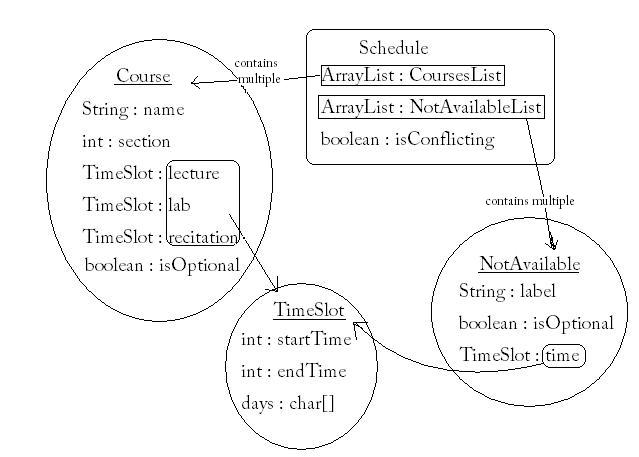
\includegraphics[scale=.50, width=140mm, height=80mm]{SRSImages/ClassOverview} 
	\end{center}

\item {\bf Operational Scenarios:}	
	\begin{itemize}
		\item Scenario One: \newline
		User starts the applet and the Intro Screen will be displayed:
			\begin{center} 
				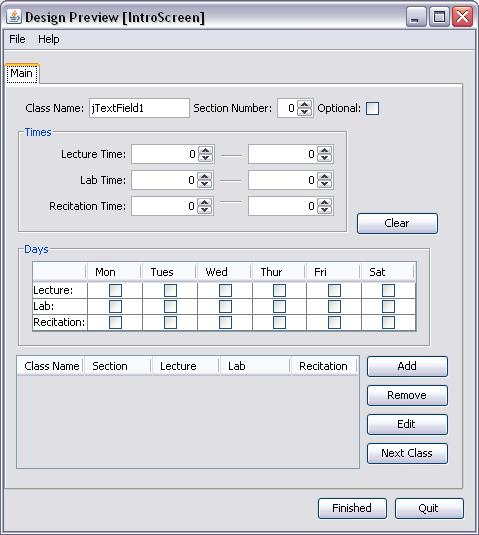
\includegraphics[scale=.50, width=70mm, height=80mm]{SRSImages/IntroScreen} 
			\end{center}
		The user fills out the form for one class. He clicks the "`add"' button and the course is added to the bottom table.  He adds some more sections for that course. Finally he clicks the "`Add Class"' button which clears the form and creates a tab containing the previous class' information. Like so:
			\begin{center} 
				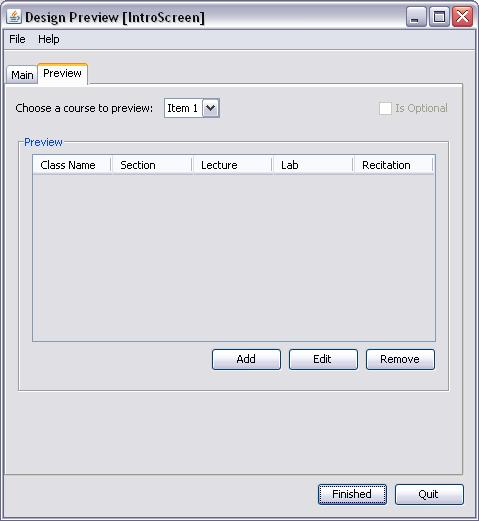
\includegraphics[scale=.50, width=70mm, height=80mm]{SRSImages/IntroScreen_Tab} 
			\end{center}
		This tab will be a preview for the user, which will allow him to look at the time slots he has added and make changes if he needs to. There will be one preview tab, in the tab the user can choose a class that he wants to preview from a drop down menu. He then adds some more classes, looks at the preview, then clicks "`Finished"'. This then takes him to the next page which asks for times that he is not available. User inputs "`Work"' for the label, sets the times and days, then clicks "`Add"' which adds that time slot to the bottom table. The page will look something like this:
			\begin{center} 
				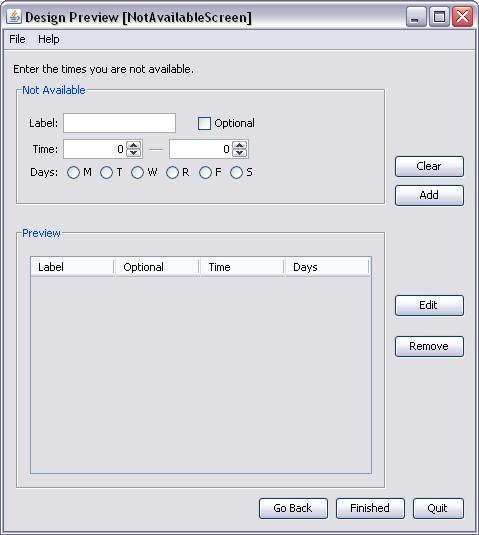
\includegraphics[scale=.50, width=70mm, height=80mm]{SRSImages/NotAvailableScreen}
			\end{center}
		User then looks at the table to make sure everything is correct then clicks "`Finished"'.  This will calculate the schedules and display the DisplayScreen which will look like this:
			\begin{center} 
				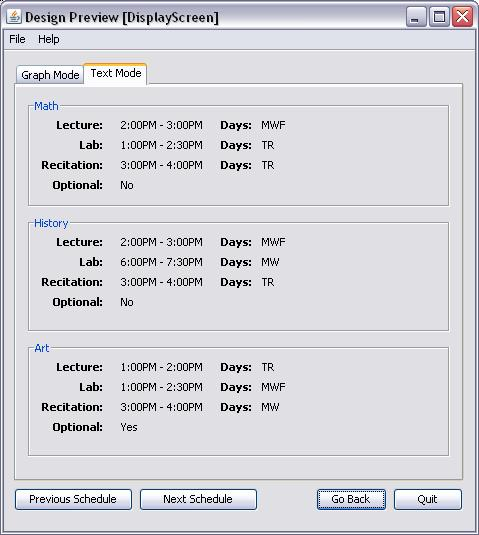
\includegraphics[scale=.50, width=70mm, height=80mm]{SRSImages/DisplayScreen_TextTab} 
			\end{center}
		User looks at the first schedule that is shown but does not like it so he clicks "`Next Schedule"' which displays another schedule in the same format. To get a better view the user clicks on Graph mode to get a visual representation of the schedule. After coming to a schedule that he likes he presses "`Quit"' to exit the program. \newline
		
		\item Scenario Two: \newline
		User starts the applet and the Intro Screen is displayed. He fills out the form for one class, but half way through he changes his mind so he clicks "`Clear"' to clear the form and begins to add another class. He adds a few sections, which are now dispayed in the table. After checking the table he finds a section that he wants to edit, so he highlights that section and clicks "`Edit"'.  This reloads all the information for that section into the form and deletes it from the table. After the user has edited it he clicks on "`Add"' and it adds it again to the list. \newline
		The user clicks "`Finished"' and is met with the NotAvailable page. The user adds some times at which he is not available. He finds that he is available on one of the times he added so he highlights it and clicks "`Remove"' to remove it from the list.  When he is done he clicks "`Finished"' which takes him to the DisplayScreen.
		Here the user can get both a visual and textual representation of his schedules. He then goes through each schedule til he finds the one he wants, writes it down, then clicks "`Quit"'.
		
		\item Scenario Three: \newline
		User starts the applet and inputs all the classes and their courses.  He looks at the preview then clicks "`Finished"'. He now inputs the times at which he is not available. He clicks "`Finished"'. The system finds no working schedules. The user decides to go back and add another Math course that might fit his schedule. The user clicks "`Go Back"' and he is met with the "`Not Available"' screen. He does not want to change anything here so he clicks "`Go Back"' and he comes to the Course preview screen. From the drop down box he selects the Math class. This displays all the possible courses for that class. 
		The user then clicks "`Add"' and this takes him to the very first page. The page is blank except for the bottom portion which displays the same courses as the ones in the preview. He inputs the information for that course then clicks "`Finished"'. He clicks "`Finished"' again to go back to the Results screen. A schedule is found and it is displayed.
		
		\item Scenario Four: \newline
		User starts the application and fills out the first form. He adds all the classes he needs but when he looks at the preview he changes his mind about one of the courses. He highlights that course and clicks "`Edit"'. This returns him to the previous tab, which is the First page. The top portion is already filled out with the information from that course. The course is deleted from the bottom section. The user edits the information he needs to then clicks "`Add"'. He then clicks "`Finished"' twice to get to the Display screen.
		
		\item Scenario Five: \newline
		User starts the application and goes fills everything out. When he gets to the last page with the results there are no working schedules. The user is willing to change his personal schedule. He clicks "`Go Back"' which takes him to the "`Not Available"' page. He highlights the time he wants to change and clicks "`Edit"'. The top panel is filled with information from this time slot and it is removed from the bottom table. He changes the information and clicks "`Add"'. When he is done he clicks "`Finished"' and the results page is Displayed. When he is satisfied he clicks "`Quit"'.
	\end{itemize}
	
	\begin{center} 
		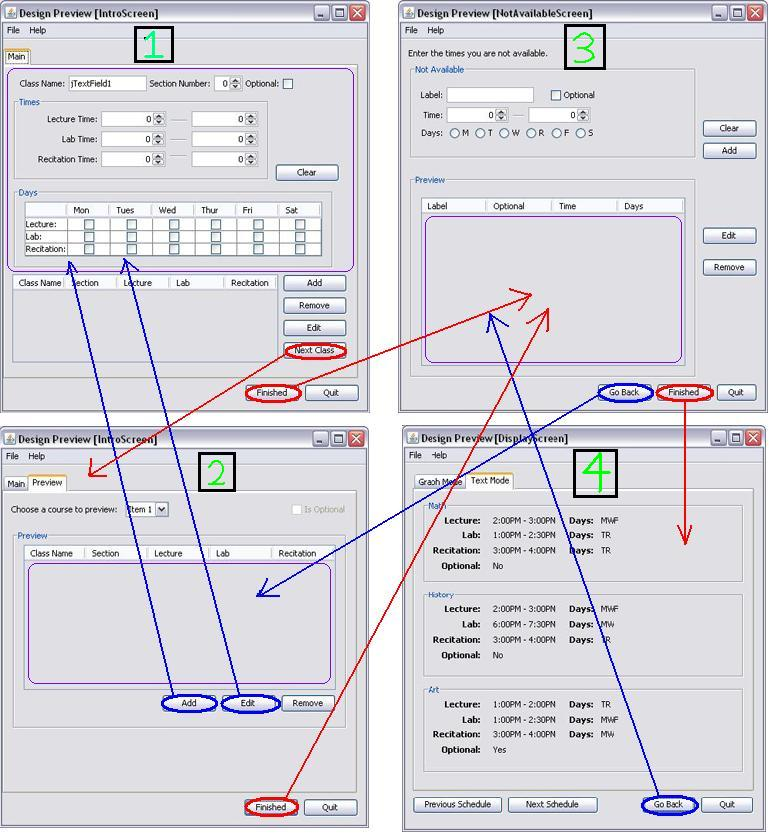
\includegraphics[scale=.05, width=140mm, height=160mm]{SRSImages/MAP2} 
	\end{center}
			
\end{enumerate}

\end{document}
